\begin{center}
  \textit{Rabah Abdul Khalek, Shaun Bailey,
    Jun Gao, Lucian Harland-Lang,  and Juan Rojo}
\end{center}

{\bf PDFs in the HL-LHC era.}
%
The detailed understanding of the quark and gluon
structure of the proton, quantified by the parton distribution functions
(PDFs)~\cite{Gao:2017yyd,Rojo:2015acz,Forte:2013wc},
is an essential ingredient for the theoretical predictions at hadron colliders.
%
PDF uncertainties represent one of the dominant theoretical systematic
errors
both for direct searches of new physics beyond the Standard
Model (bSM)~\cite{Beenakker:2015rna}
as well as in
the profiling of the Higgs boson sector~\cite{deFlorian:2016spz}.
%
Therefore, improving our knowledge of the proton structure
is an essential task for the high-precision physics
program to be carried out at future runs of the LHC, including
the HL-LHC era.

Modern global PDF fits~\cite{Ball:2017nwa,Dulat:2015mca,
  Harland-Lang:2014zoa,Alekhin:2017kpj}
include a wide range of LHC measurements in
processes such as the production of jets, weak gauge bosons,
and top quark pairs, among others.
%
Recent breakthroughs in the calculation
of NNLO QCD and NLO QED and electroweak corrections to
most PDF-sensitive processes have been instrumental in
allowing for the full exploitation of the information provided by the LHC measurements.
%
The impact of high-precision LHC data combined with state-of-the art
perturbative calculations has been quantified for many of the processes
of interest, such as top-quark pair production~\cite{Czakon:2016olj,Guzzi:2014wia},
the transverse momentum spectrum of $Z$ bosons~\cite{Boughezal:2017nla}, 
direct photon production~\cite{d'Enterria:2012yj,Campbell:2018wfu},
$D$ meson production in the forward region~\cite{Gauld:2015yia,Zenaiev:2015rfa,Gauld:2016kpd}, $W$ production
in association with charm quarks~\cite{Aad:2014xca,Chatrchyan:2013mza,CMS-PAS-SMP-17-014},
and inclusive jet production~\cite{Currie:2016bfm,Rojo:2014kta}.

From the point of view of PDF determinations, the availability of the
immense data samples at the HL-LHC
will permit a significant extension
of the kinematic coverage of PDF-sensitive measurements
as well as a marked improvement in their statistical and systematic uncertainties.
%
In this contribution, we summarise the main results
of our PDF projections for the HL-LHC era presented
in~\cite{Khalek:2018mdn}.
%
The main idea is to quantify the impact of the future HL--LHC
measurements on the proton PDFs and their
uncertainties, with emphasis on
their implications for Higgs physics.
%
Specifically, we quantify the 
constraints of the HL--LHC pseudo-data
on the PDF4LHC15
set~\cite{Butterworth:2015oua,Gao:2013bia,Carrazza:2015hva,Carrazza:2015aoa}
by means
of the Hessian Profiling
method~\cite{Paukkunen:2014zia} (see also~\cite{Schmidt:2018hvu}).
%
We choose the PDF4LHC15 set since it broadly represents
the state-of-the-art understanding of
the proton structure.

In Fig.~\ref{fig:kinHLLHC} we show the
kinematical coverage in the $(x,Q^2)$ plane of the
  HL--LHC pseudo-data included in this analysis.
  %
  As indicated there, we have simulated pseudo-data for
  the following processes: top quark pair production,
  high-mass and forward Drell-Yan $W,Z$ production, direct
  photon and inclusive jet production, the transverse momentum
  of $Z$ bosons, and the production of $W$ bosons in association
  with charm quarks.
  %
  The HL--LHC pseudo-data therefore spans a wide region in the kinematic
  plane, namely $6\times 10^{-5} < x < 0.7$ and
  $40~{\rm GeV} < Q < 7~{\rm TeV}$.
  %
  In particular, one sees that the HL-LHC coverage of the large-$x$ region,
  where current PDF fits exhibit large uncertainties,
  is markedly improved as compared to available LHC
  measurements.
  
%%%%%%%%%%%%%%%%%%%%%%%%%%%%%%%%%%%%%%%%%%%%%%%%%%%%%%%%%%%%%%%%%%%%%%%%%
\begin{figure}[t]
\centering
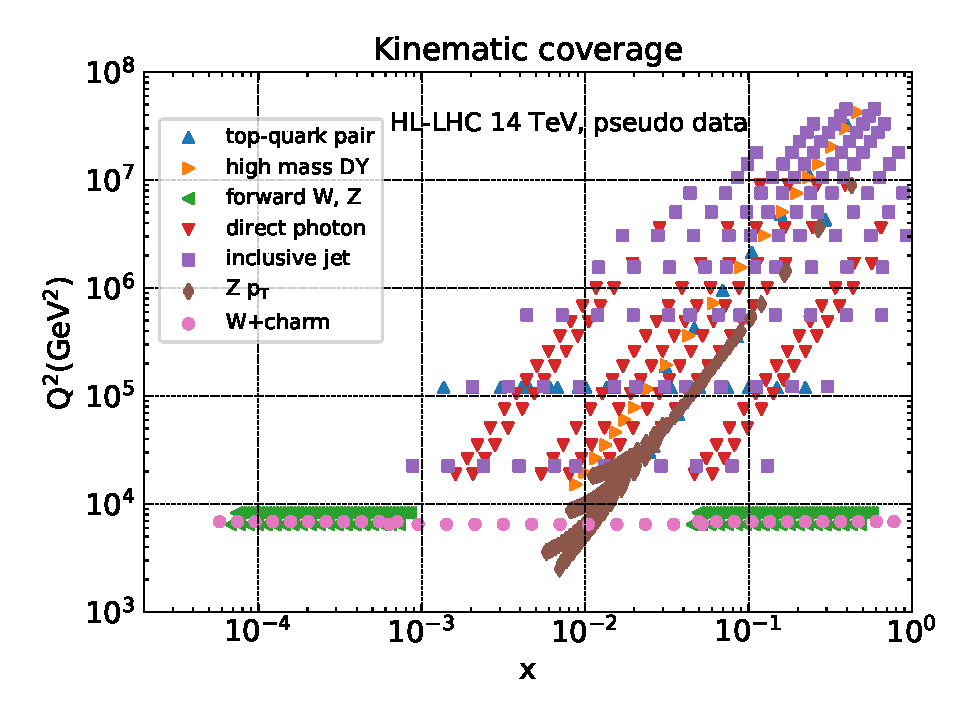
\includegraphics[width=0.67\textwidth]{\main/section2/plots/kinHLLHC.pdf}
\caption{\small 
  The kinematical coverage in the $(x,Q^2)$ plane of the
  HL--LHC pseudo-data.
 \label{fig:kinHLLHC}} 
\end{figure}
%%%%%%%%%%%%%%%%%%%%%%%%%%%%%%%%%%%%%%%%%%%%%%%%%%%%%%%%%%%%%%%%%%%%%%%%%%

{\bf Results.}
%
As an illustration of the impact of individual sets
of HL-LHC pseudo-data,
in Fig.~\ref{fig:resultsPDFs.pdf} we show 
the comparison between the HL--LHC projected measurements
and the theoretical predictions for the lepton
rapidity distribution in forward $W+$charm production
  and for the invariant mass $m_{t\bar{t}}$ distribution in top-quark
  pair production. These two particular datasets probe the poorly-known strange quark and
  the gluon at large-$x$, respectively.
  %
   The theory calculations are shown both before (PDF4LHC15)
   and after profiling.
   %
  In the bottom panel, we show the same results normalised
  to the central value of the original theory calculation.
  %
  In both cases we see that the expected precision of the HL-LHC
  measurements is rather higher than the current PDF uncertainties,
  and therefore we observe a marked improvement once they
  are included in PDF4LHC15 via the Hessian profiling.
  

%%%%%%%%%%%%%%%%%%%%%%%%%%%%%%%%%%%%%%%%%%%%%%%%%%%%%%%%%%%%%%%%%%%%%
\begin{figure}[t]
  \begin{center}
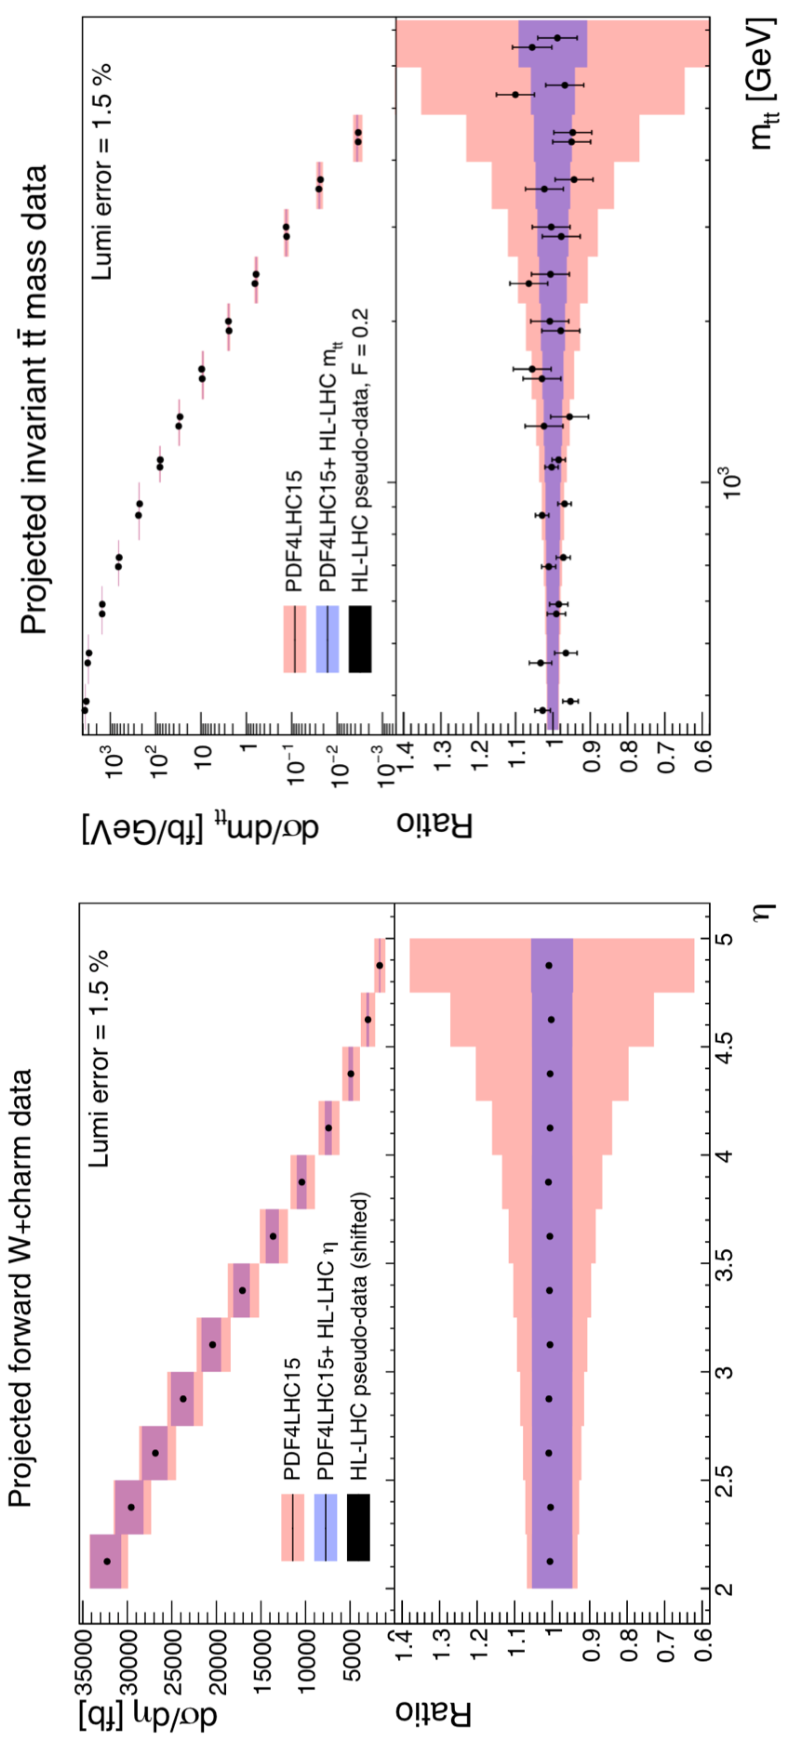
\includegraphics[width=0.44\linewidth,angle=-90]{\main/section2/plots/resultsPDFs.pdf}
\caption{\small Comparison between the HL--LHC pseudo-data
  and the theoretical predictions for forward $W+$charm production (left)
  and for the invariant mass $m_{t\bar{t}}$ distribution in top-quark
  pair production (right).
  %
   The theory calculations are shown both before (PDF4LHC15)
   and after profiling.
   %
       \label{fig:resultsPDFs.pdf} }
  \end{center}
\end{figure}
%%%%%%%%%%%%%%%%%%%%%%%%%%%%%%%%%%%%%%%%%%%%%%%%%%%%%%%%%%%%%%%%%%%%%%

In this study we have considered three
different scenarios for the
experimental systematic uncertainties of the HL--LHC pseudo-data.
     %
    These scenarios, ranging from more conservative to more optimistic, differ among them in
    the reduction factor
    applied to the systematic errors of the reference
    8 TeV or 13 TeV measurements, see~\cite{Khalek:2018mdn}
    for more details.
    %
    In particular, in the optimistic scenario we assume a reduction
    of the systematic errors by a factor 2.5 (5) as compared to the
    reference 8 TeV (13 TeV) measurements, while for
    the conservative scenario we assume no reduction in systematic
    errors with respect to the 8 TeV reference.
    %
    Reassuringly, we obtain that the main results of our
    study depend only mildly in the specific assumption for
    the values of this reduction factor.

    In Fig.~\ref{fig:PDFratios}  we compare the PDF4LHC15 set
    with the strange quark and gluon PDFs obtained once the entire
    set of HL-LHC pseudo-data summarised in Fig.~\ref{fig:kinHLLHC}
    has been included via profiling.
    %
    We show results both in the conservative (A) and optimistic (C) scenarios
    for the projections of the experimental systematic uncertainties.
    %
    We observe that the
  impact of the HL--LHC pseudo-data is reasonably similar
  in both scenarios.
  %
  This is due to the fact that we have chosen
  those processes which will benefit from a significant improvement in statistics, independent of the specific assumption about the systematic errors. These then tend to lie in kinematic regions where the PDFs themselves are generally less
  well determined.
  %
  We also observe
  a marked reduction of the PDF uncertainties in all cases.
  %
  In the case of the gluon PDF, there is an improvement of
  uncertainties in the complete relevant range of momentum
  fraction $x$.
  %
  This is a direct consequence of the fact that
  we have included several HL--LHC processes
  that have direct sensitivity to the gluon
  content of the proton, including jet, direct photon, and top quark pair
  production, as well as the transverse momentum of $Z$ bosons.
  %
  As we discuss next, this has direct implications for the phenomenology of Higgs
  boson production.
      
%%%%%%%%%%%%%%%%%%%%%%%%%%%%%%%%%%%%%%%%%%%%%%%%%%%%%%%%%%%%%%%%%%%%%
\begin{figure}[t]
  \begin{center}
    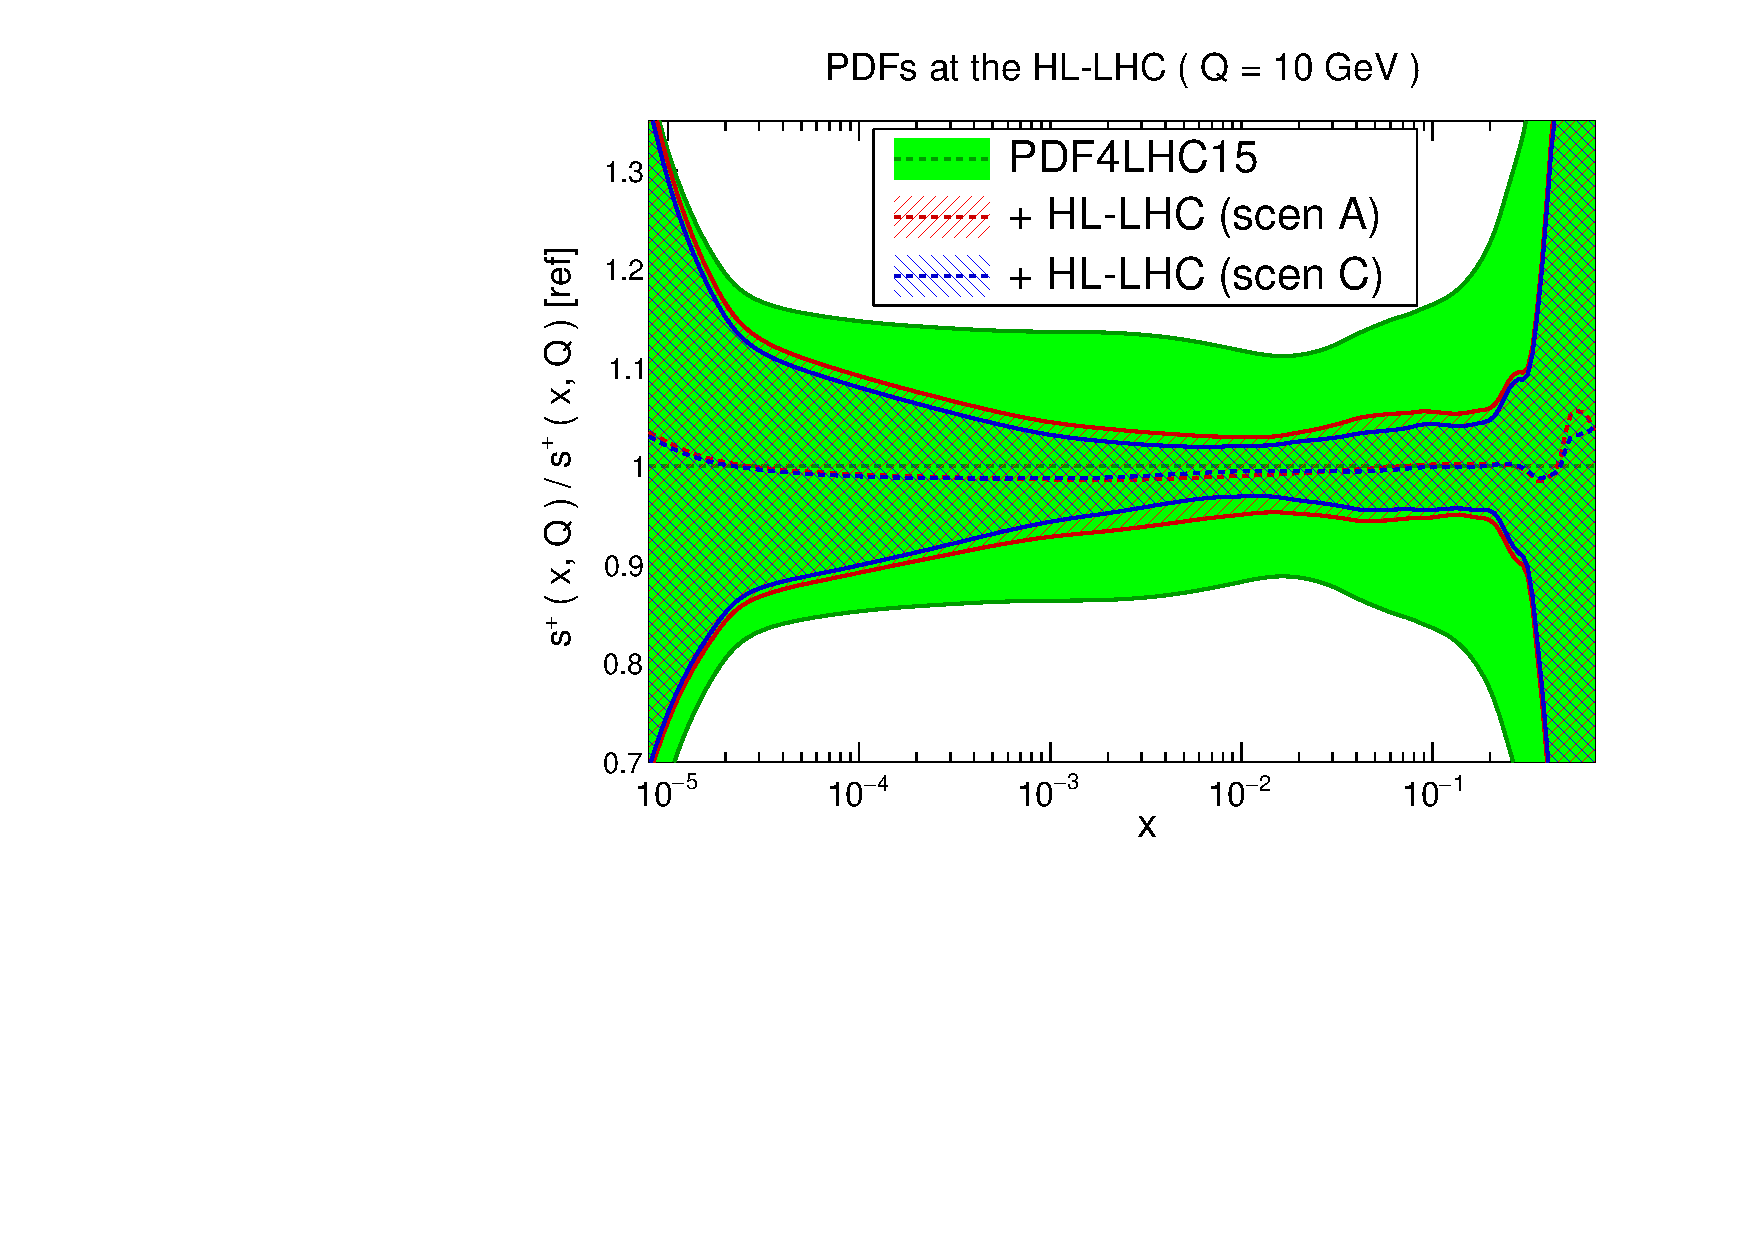
\includegraphics[width=0.49\linewidth]{\main/section2/plots/xsp-hllhc.pdf}
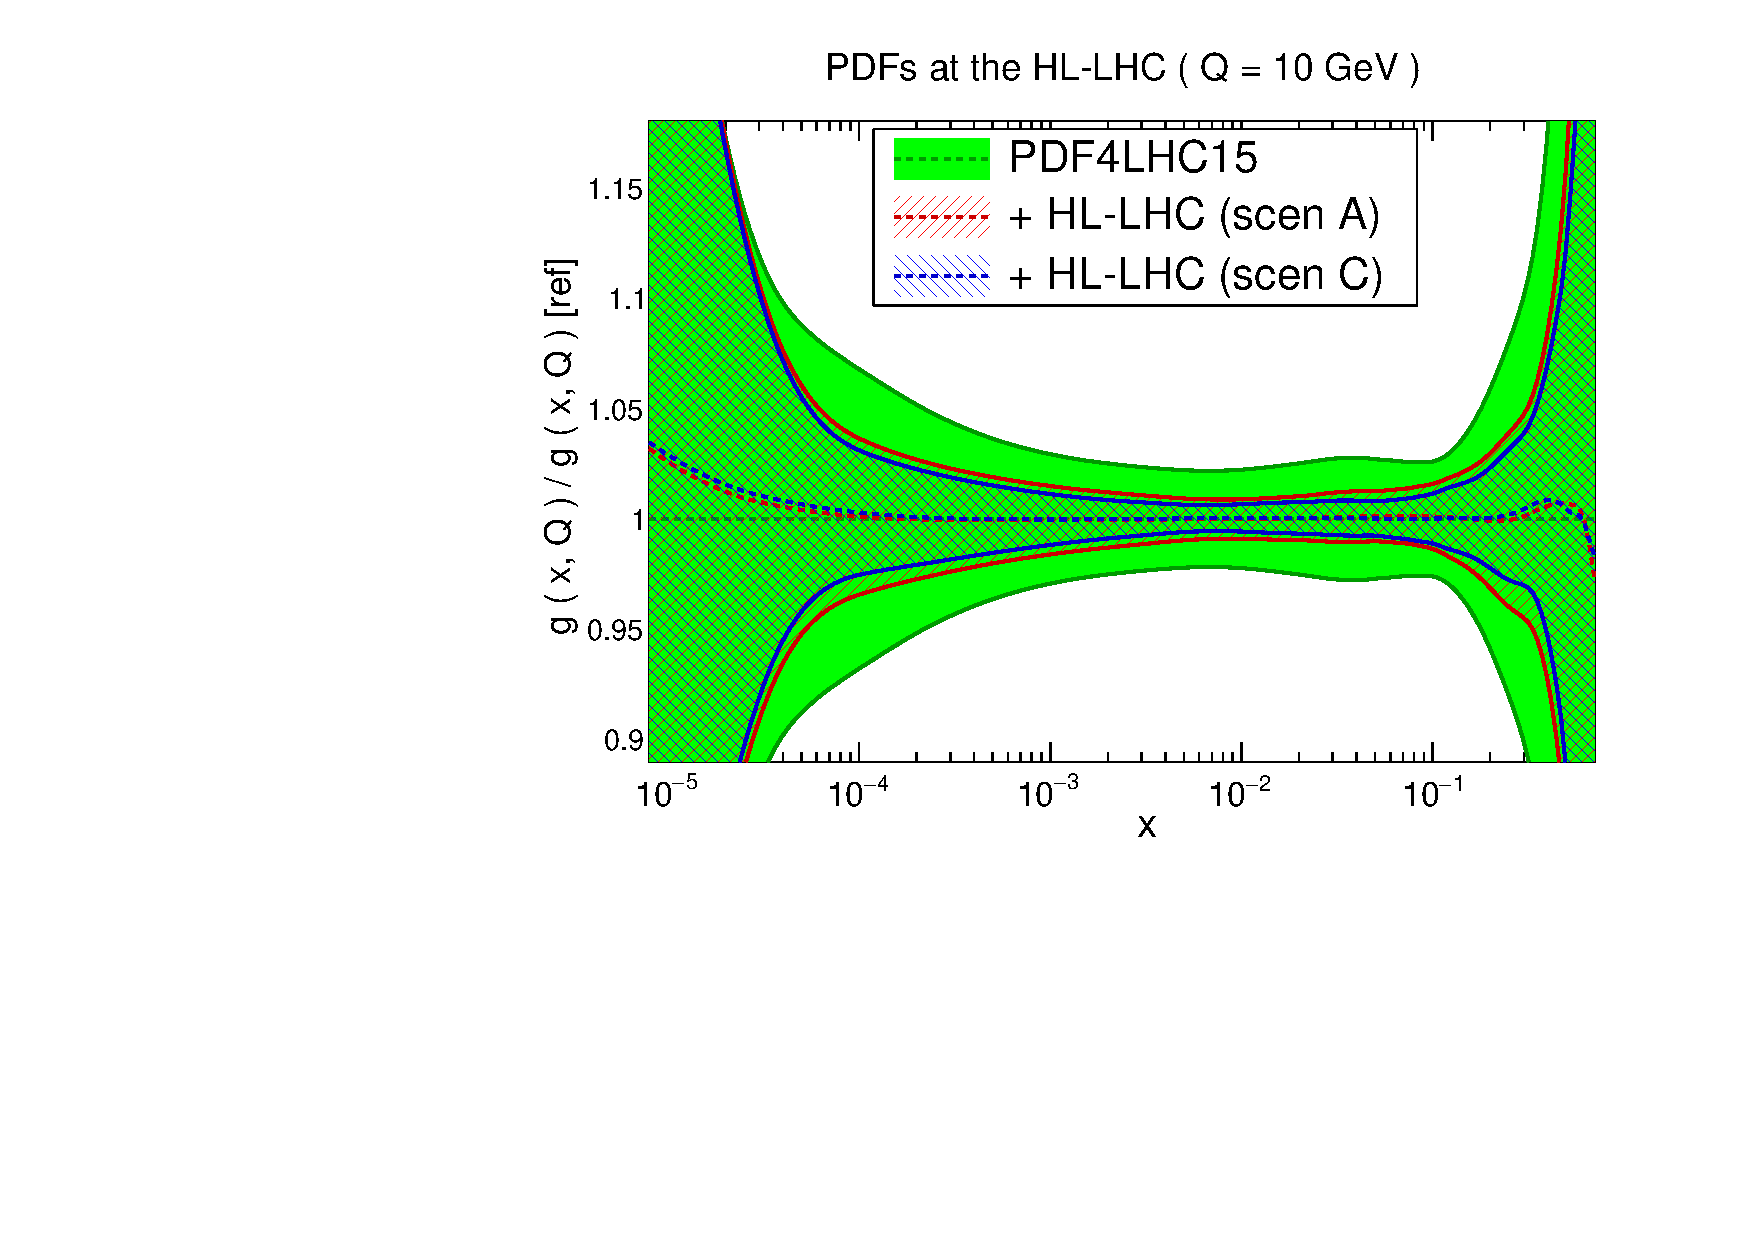
\includegraphics[width=0.49\linewidth]{\main/section2/plots/xg-hllhc.pdf}
\caption{\small Comparison of the PDF4LHC15 set with the profiled sets
  with HL--LHC pseudo-data.
  %
  We show the strange (left) and gluon (right) PDFs
  normalized to the central value of
  the baseline.
     \label{fig:PDFratios} }
  \end{center}
\end{figure}
%%%%%%%%%%%%%%%%%%%%%%%%%%%%%%%%%%%%%%%%%%%%%%%%%%%%%%%%%%%%%%%%%%%%%%

{\bf Implications for Higgs physics.}
%
In Table~\ref{fig:PDFs-HL--LHC-summaryTable} we indicate
the reduction of the PDF uncertainties
in comparison to the PDF4LHC15 baseline for
different initial partonic combinations (that is, a value
of 1 corresponds to no improvement).
  %
  Results are presented for three different bins
  of the invariant mass $M_X$ of the produced system for
  the three initial states relevant for Higgs production:
  gluon-gluon (for $gg\to h$ and $t\bar{t}h$), quark-quark
  (for vector boson fusion) and quark-antiquark
  (for associated $Wh$ and $Zh$ production).
  %
  The values shown outside (inside) the brackets correspond to the
  optimistic (conservative) scenario.
  %
  We can see that for the $M_X$ region relevant for the SM Higgs
  boson production, as well as for related bSM Higgs-like scalars, namely
  $40~{\rm GeV}\le M_X\le 1~{\rm TeV}$, the HL-LHC pseudo-data leads
  to a reduction by almost a factor four in the optimistic scenario
  in the $gg$ channel, and around a factor three in the $q\bar{q}$
  and $qq$ channels.
  %
  This implies that precision calculations of Higgs production
  at the HL-LHC should be possible with significantly reduced PDF
  uncertainties compared to current state-of-the-art predictions.
  
%%%%%%%%%%%%%%%%%%%%%%%%%%%%%%%%%%%%%%%%%%%%%%%%%%%%%%%%%%%%%%%%%%%%%
\begin{table}[t]
  \begin{center}
  \small
   \renewcommand{\arraystretch}{1.70}
\begin{tabular}{c|c|c|c}
\toprule
Ratio to baseline  & $10~{\rm GeV}\le M_X\le 40~{\rm GeV}$   &
 $40~{\rm GeV}\le M_X\le 1~{\rm TeV}$&
  $1~{\rm TeV}\le M_X\le 6~{\rm TeV}$\\
\midrule
gluon-gluon & 0.50 (0.60)  & 0.28 (0.40)  & 0.22 (0.34)     \\
quark-quark &  0.74 (0.79) & 0.37 (0.46) &  0.43 (0.59)     \\
quark-antiquark & 0.71 (0.76) & 0.31 (0.40)  &  0.50 (0.60)     \\
\bottomrule
\end{tabular}
\vspace{+0.4cm}
\caption{\small The reduction of the PDF uncertainties
as compared to the PDF4LHC15 baseline for
different initial partonic combinations in the 
  optimistic (conservative) scenario.
     \label{fig:PDFs-HL--LHC-summaryTable}
 }
  \end{center}
\end{table}
%%%%%%%%%%%%%%%%%%%%%%%%%%%%%%%%%%%%%%%%%%%%%%%%%%%%%%%%%%%%%%%%%%%%%%

To illustrate this improvement, in Fig.~\ref{fig:MCFMxsects}
we present the comparison of the predictions for 
    SM Higgs production at $\sqrt{s}=14$ TeV between the PDF4LHC15
    baseline and the profiled PDF sets.
    %
    Specificially, we show
     Higgs boson production in gluon fusion with heavy top
      quark effective theory, both inclusive
      and decaying into $b\bar{b}$ as a function of $p_T^{b,\rm min}$ (left), and
      then in association with a hard jet as a function of its transverse
      momentum $p_{\rm T}^{\rm jet, min}$ (right).
      %
      The calculations have been performed using {\tt MCFM8.2} with leading-order
      matrix elements.
      %
      The marked reduction of PDF uncertainties is consistent with
      the values reported in Table~\ref{fig:PDFs-HL--LHC-summaryTable}.
     

%%%%%%%%%%%%%%%%%%%%%%%%%%%%%%%%%%%%%%%%%%%%%%%%%%%%%%%%%%%%%%%%%%%%%
\begin{figure}[t]
  \begin{center}
    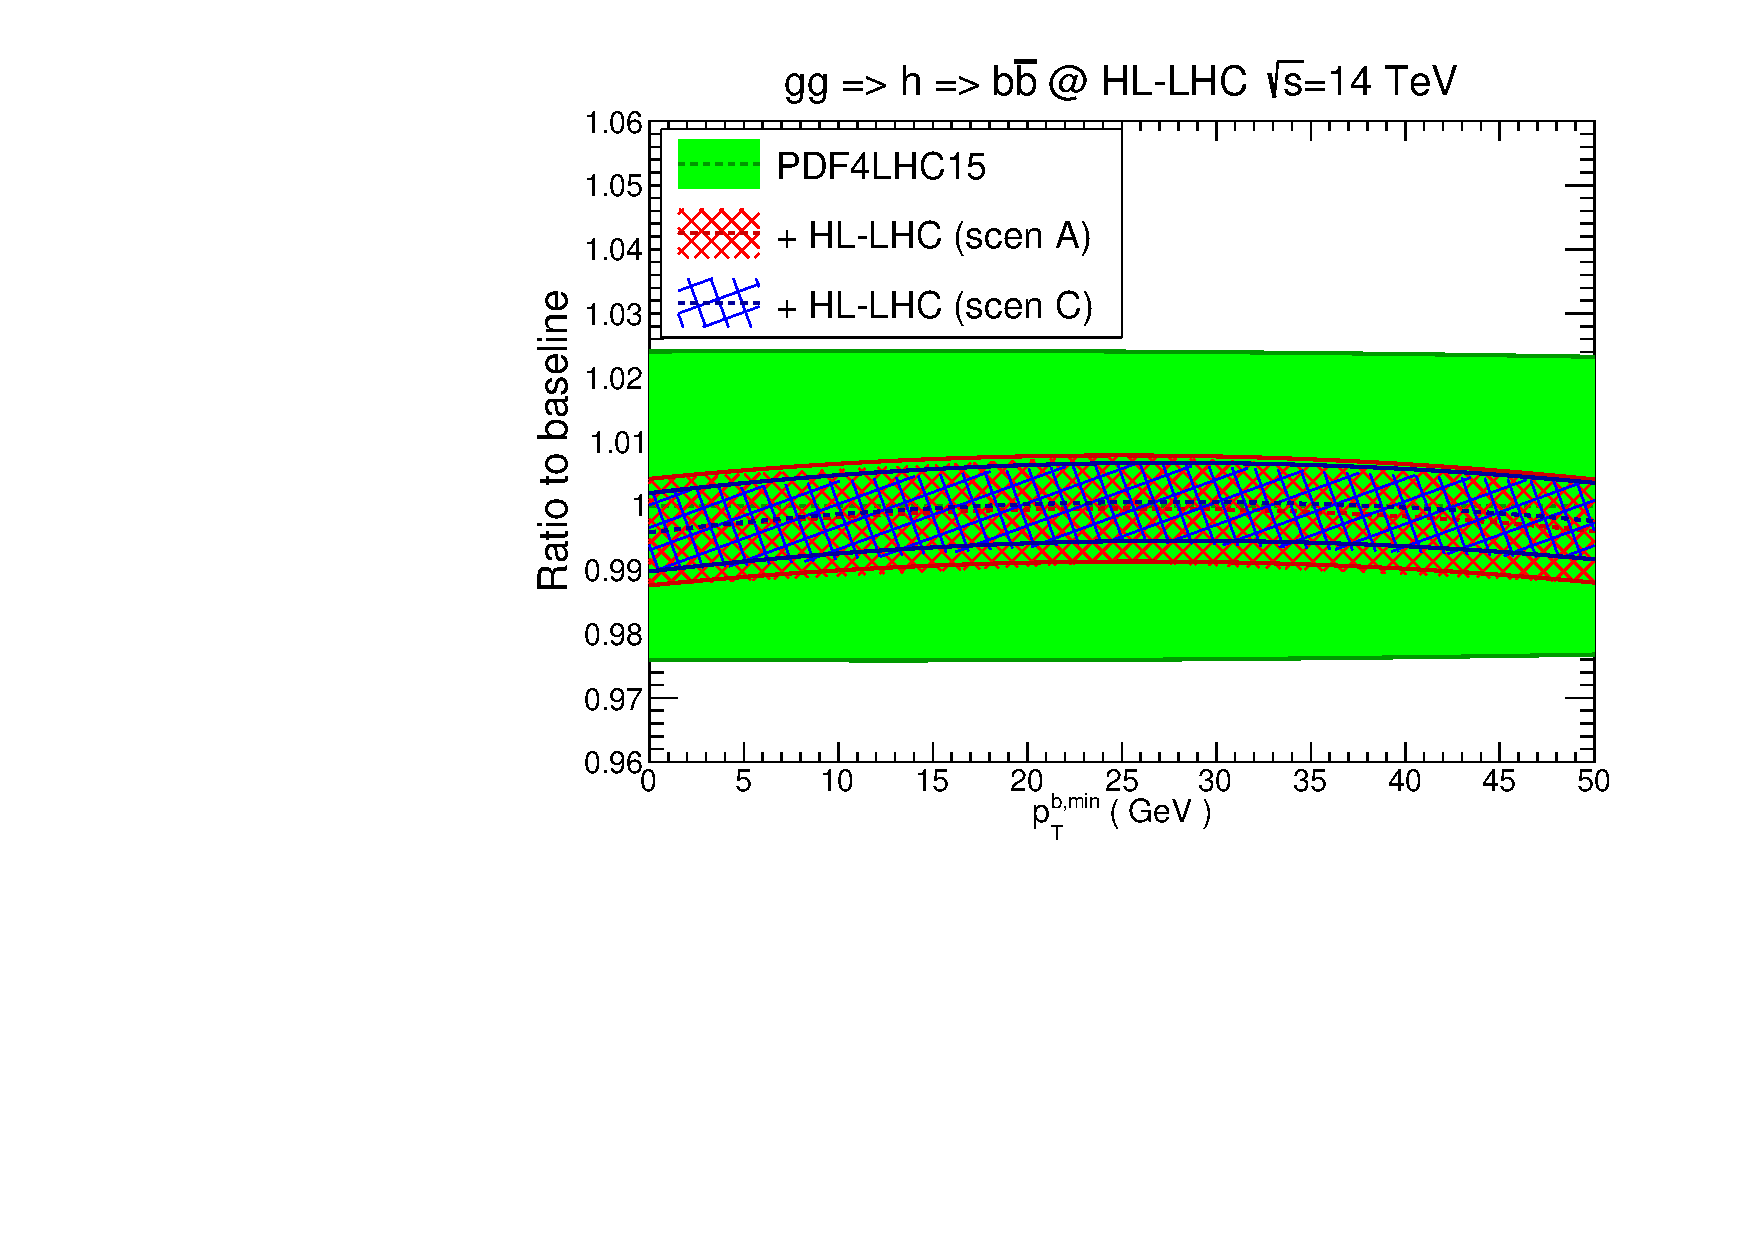
\includegraphics[width=0.49\linewidth]{\main/section2/plots/ggHiggs.pdf}
    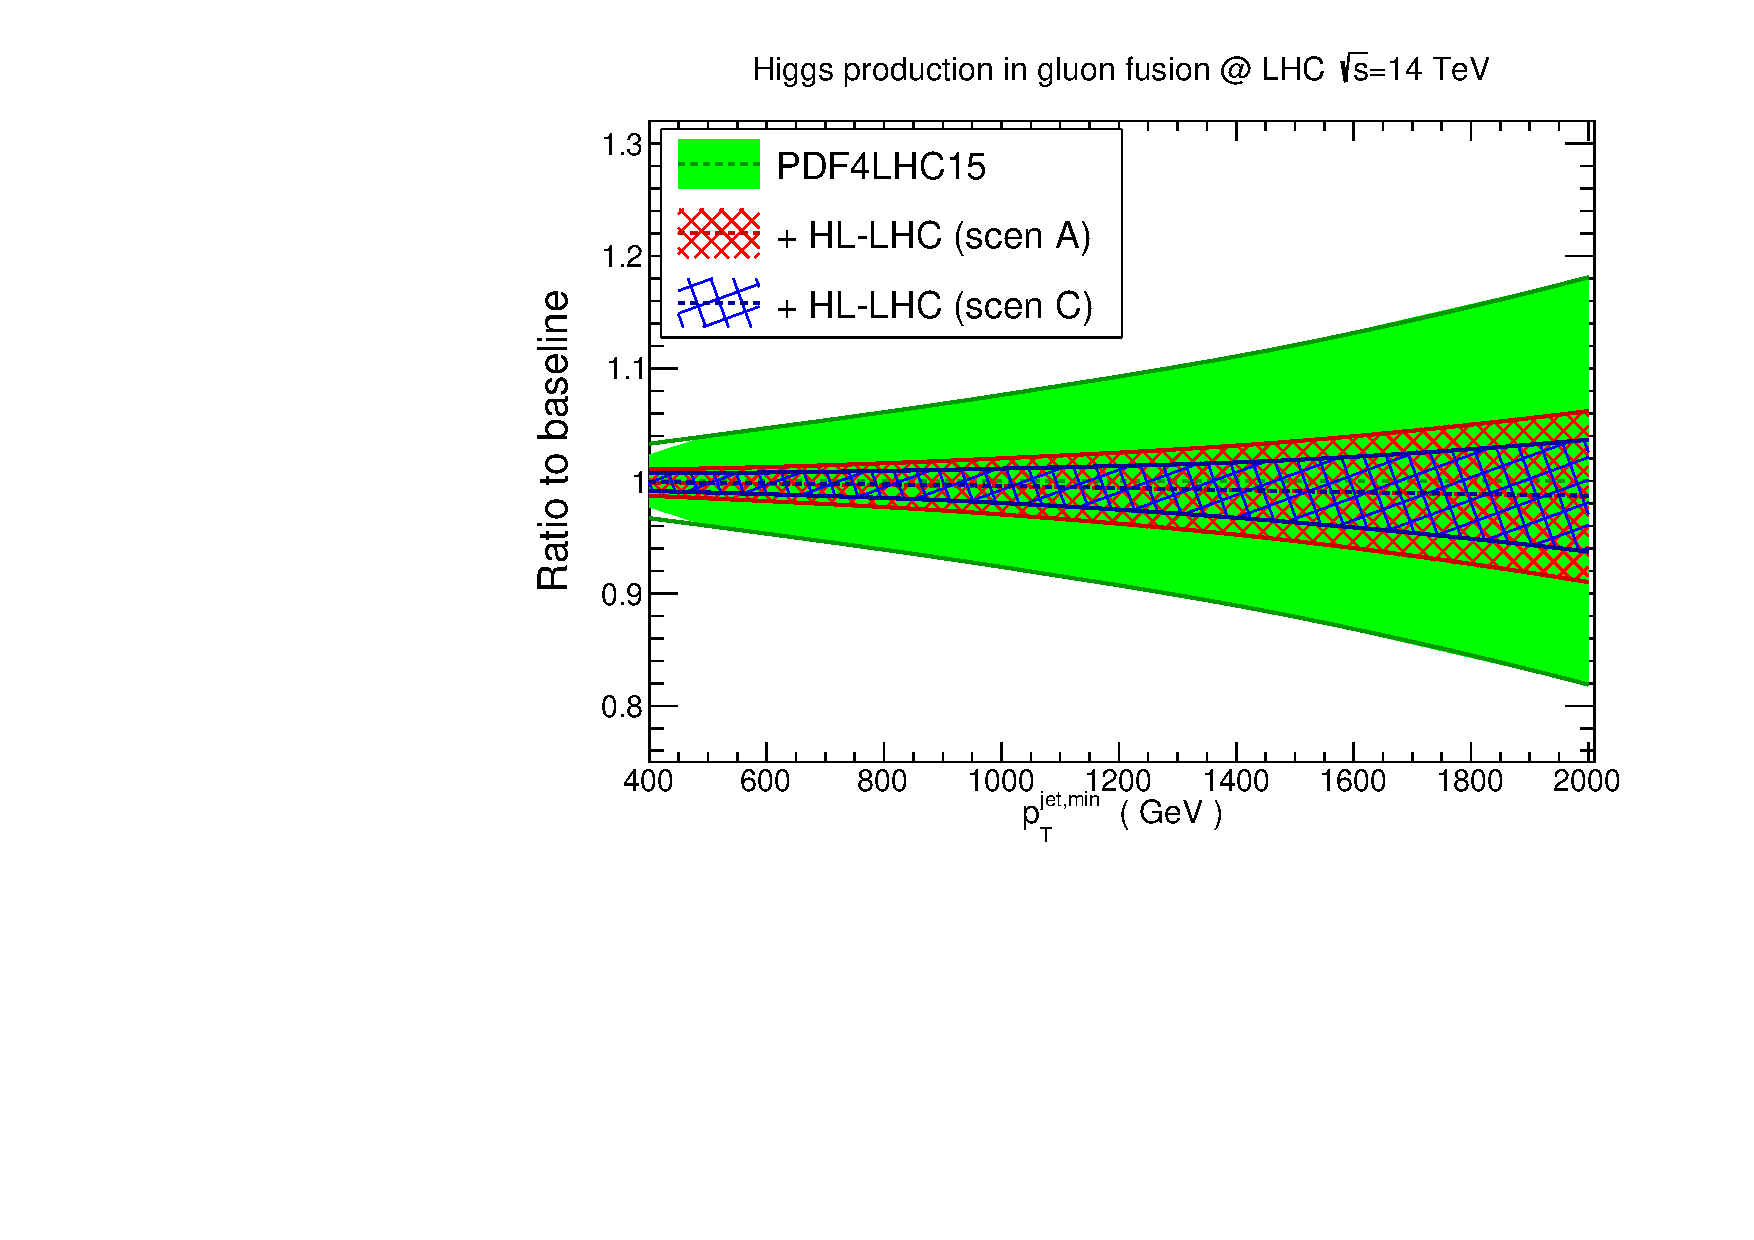
\includegraphics[width=0.49\linewidth]{\main/section2/plots/HiggsJet.pdf}
    \caption{\small Comparison of the predictions for 
    SM Higgs production cross-sections at $\sqrt{s}=14$ TeV between the PDF4LHC15
baseline and the profiled PDF sets with HL--LHC pseudo--data.
     \label{fig:MCFMxsects} }
  \end{center}
\end{figure}
%%%%%%%%%%%%%%%%%%%%%%%%%%%%%%%%%%%%%%%%%%%%%%%%%%%%%%%%%%%%%%%%%%%%%%
 
      Finally, there are two caveats to be added concerning this study.
      %
      First we have only considered a subset of all possible measurements of relevance for PDF fits at HL--LHC.
      %
      Second, possible data incompatibility has not been
      accounted for fully. These may strengthen and weaken, respectively, the constraining powers of future LHC data on PDFs.
      %
      
The results of this study are made
 publicly available in the {\tt LHAPDF6} format~\cite{Buckley:2014ana},
 for the three
 scenarios that have been considered, and can be
 downloaded from:
 \begin{center}
{\tt  https://data.nnpdf.science/HLLHC\_YR/PDF4LHC15\_nnlo\_hllhc\_scen1.tgz}\\
{\tt https://data.nnpdf.science/HLLHC\_YR/PDF4LHC15\_nnlo\_hllhc\_scen2.tgz}\\
{\tt https://data.nnpdf.science/HLLHC\_YR/PDF4LHC15\_nnlo\_hllhc\_scen3.tgz}
\end{center}


%%%%%%%%%%%%%%%%%%%%%%%%%%%%%%%%%%%%%%%%%%%%%%%%%%%
%%%%%%%%%%%%%%%%%%%%%%%%%%%%%%%%%%%%%%%%%%%%%%%%%%%
